% Options for packages loaded elsewhere
\PassOptionsToPackage{unicode}{hyperref}
\PassOptionsToPackage{hyphens}{url}
\PassOptionsToPackage{dvipsnames,svgnames,x11names}{xcolor}
%
\documentclass[
  letterpaper,
  DIV=11,
  numbers=noendperiod]{scrartcl}

\usepackage{amsmath,amssymb}
\usepackage{iftex}
\ifPDFTeX
  \usepackage[T1]{fontenc}
  \usepackage[utf8]{inputenc}
  \usepackage{textcomp} % provide euro and other symbols
\else % if luatex or xetex
  \usepackage{unicode-math}
  \defaultfontfeatures{Scale=MatchLowercase}
  \defaultfontfeatures[\rmfamily]{Ligatures=TeX,Scale=1}
\fi
\usepackage{lmodern}
\ifPDFTeX\else  
    % xetex/luatex font selection
\fi
% Use upquote if available, for straight quotes in verbatim environments
\IfFileExists{upquote.sty}{\usepackage{upquote}}{}
\IfFileExists{microtype.sty}{% use microtype if available
  \usepackage[]{microtype}
  \UseMicrotypeSet[protrusion]{basicmath} % disable protrusion for tt fonts
}{}
\makeatletter
\@ifundefined{KOMAClassName}{% if non-KOMA class
  \IfFileExists{parskip.sty}{%
    \usepackage{parskip}
  }{% else
    \setlength{\parindent}{0pt}
    \setlength{\parskip}{6pt plus 2pt minus 1pt}}
}{% if KOMA class
  \KOMAoptions{parskip=half}}
\makeatother
\usepackage{xcolor}
\setlength{\emergencystretch}{3em} % prevent overfull lines
\setcounter{secnumdepth}{-\maxdimen} % remove section numbering
% Make \paragraph and \subparagraph free-standing
\ifx\paragraph\undefined\else
  \let\oldparagraph\paragraph
  \renewcommand{\paragraph}[1]{\oldparagraph{#1}\mbox{}}
\fi
\ifx\subparagraph\undefined\else
  \let\oldsubparagraph\subparagraph
  \renewcommand{\subparagraph}[1]{\oldsubparagraph{#1}\mbox{}}
\fi


\providecommand{\tightlist}{%
  \setlength{\itemsep}{0pt}\setlength{\parskip}{0pt}}\usepackage{longtable,booktabs,array}
\usepackage{calc} % for calculating minipage widths
% Correct order of tables after \paragraph or \subparagraph
\usepackage{etoolbox}
\makeatletter
\patchcmd\longtable{\par}{\if@noskipsec\mbox{}\fi\par}{}{}
\makeatother
% Allow footnotes in longtable head/foot
\IfFileExists{footnotehyper.sty}{\usepackage{footnotehyper}}{\usepackage{footnote}}
\makesavenoteenv{longtable}
\usepackage{graphicx}
\makeatletter
\def\maxwidth{\ifdim\Gin@nat@width>\linewidth\linewidth\else\Gin@nat@width\fi}
\def\maxheight{\ifdim\Gin@nat@height>\textheight\textheight\else\Gin@nat@height\fi}
\makeatother
% Scale images if necessary, so that they will not overflow the page
% margins by default, and it is still possible to overwrite the defaults
% using explicit options in \includegraphics[width, height, ...]{}
\setkeys{Gin}{width=\maxwidth,height=\maxheight,keepaspectratio}
% Set default figure placement to htbp
\makeatletter
\def\fps@figure{htbp}
\makeatother

\usepackage[dvipsnames]{xcolor}
\definecolor{myblue}{rgb}{0.592, 0.737, 0.878}
\setkomafont{title}{\normalfont\large\color{myblue}}
\setkomafont{section}{\normalfont\large\color{myblue}}
\setkomafont{subsection}{\normalfont\normalsize\color{myblue}}
\KOMAoption{captions}{tableheading}
\makeatletter
\@ifpackageloaded{caption}{}{\usepackage{caption}}
\AtBeginDocument{%
\ifdefined\contentsname
  \renewcommand*\contentsname{Table of contents}
\else
  \newcommand\contentsname{Table of contents}
\fi
\ifdefined\listfigurename
  \renewcommand*\listfigurename{List of Figures}
\else
  \newcommand\listfigurename{List of Figures}
\fi
\ifdefined\listtablename
  \renewcommand*\listtablename{List of Tables}
\else
  \newcommand\listtablename{List of Tables}
\fi
\ifdefined\figurename
  \renewcommand*\figurename{Figure}
\else
  \newcommand\figurename{Figure}
\fi
\ifdefined\tablename
  \renewcommand*\tablename{Table}
\else
  \newcommand\tablename{Table}
\fi
}
\@ifpackageloaded{float}{}{\usepackage{float}}
\floatstyle{ruled}
\@ifundefined{c@chapter}{\newfloat{codelisting}{h}{lop}}{\newfloat{codelisting}{h}{lop}[chapter]}
\floatname{codelisting}{Listing}
\newcommand*\listoflistings{\listof{codelisting}{List of Listings}}
\makeatother
\makeatletter
\makeatother
\makeatletter
\@ifpackageloaded{caption}{}{\usepackage{caption}}
\@ifpackageloaded{subcaption}{}{\usepackage{subcaption}}
\makeatother
\ifLuaTeX
  \usepackage{selnolig}  % disable illegal ligatures
\fi
\usepackage[style=nature,]{biblatex}
\addbibresource{My Library.bib}
\usepackage{bookmark}

\IfFileExists{xurl.sty}{\usepackage{xurl}}{} % add URL line breaks if available
\urlstyle{same} % disable monospaced font for URLs
\hypersetup{
  pdftitle={Upgrade Proposal},
  colorlinks=true,
  linkcolor={blue},
  filecolor={Maroon},
  citecolor={Blue},
  urlcolor={Blue},
  pdfcreator={LaTeX via pandoc}}

\title{Upgrade Proposal}
\author{Julia Marcinkowska \and  \and }
\date{}

\begin{document}
\maketitle

\section{Background}\label{background}

\emph{Summary of current state of the field and context within which the
research is located, covering current theory/state of the evidence and
referring to relevant literature (500-1,000 words).}

The NMDA hypofunction hypothesis of schizophrenia proposes that
decreased activity of NMDA receptors has a key role in the development
of schizophrenia pathology. The affected NMDA receptors are primarily
localised at GABAergic fast-spiking PV
interneurons\autocite{nakazawa_spatial_2017}; where decreased activity
of PV interneurons causes a disinhibition of their activity on pyramidal
neurons, disrupting the excitation-inhibition (E/I) balance, and leading
to increased excitation. MR spectroscopy studies report increased
glutamate in the ACC, hippocampus, and other medial temporal cortical
regions
\autocite{merritt_nature_2017,kraguljac_increased_2013,marsman_glutamate_2013}.
Hyperactivity in the hippocampus is observed in the early stages in
schizophrenia, as well as in people at clinical high risk of
schizophrenia that subsequently develop the disorders, suggesting that
increased glutamatergic activity in this region might be implicated in
the development of the pathology at early stages of the disorder, and
later contribute to hyperdopaminergia in the striatum. This is
consistent with the observations that administation of {NMDA}
antagonists like phencyclidine and ketamine induces behaviours
comparable to all three schizoprenia symptom dimensions (positive,
negative, and cognitive symptoms)\autocite{beck_association_2020}, and
repeated administration results in increased release of {DA} in rodent
striatum\autocite{balla_continuous_2001}, suggesting that
hyperdopaminergia is caused by decreased {NMDA} activity
\autocite{grace_dopamine_2012,grace_dysregulation_2016}. The role of
NMDA hypofunction in the early stages of schizophrenia makes it an
important target of translationsal research.

Alterations in synaptic function have also been implicated in the
aetiology of schizophrenia \autocite{howes_synaptic_2023} and are
thought to be related to the E/I imbalance. Excitotoxicity caused by
increased glutamatergic activity might be one of the contributing
factors in the reduction in synaptic connections in schizophrenia
\autocite{glantz_apoptotic_2006}. Post-mortem studies report decreased
levels of synaptic proteins \autocite{osimo_synaptic_2019}, supporting
the theory of alteration in synaptic density. Recent advatages in PET
imaging have enabled in-vivo imaging of synaptic density. By using a
radiotracer selective for the synaptic vesicle glycoprotein 2A (SV2A),
localised in the pre-synaptic terminals, SV2A density can be a proxy for
measuring synaptic densisty. Human SV2A PET studies reported decreased
levels of SV2A in people with schizophrenia
\autocite{radhakrishnan_vivo_2021,onwordi_synaptic_2020} and an altered
relationship glutamate and synaptic function
\autocite{onwordi_relationship_2021}. In healthy participants there is a
positive correlation between SV2A density and glutamate in ACC and
hippocampus, but no significant correlations were found in
schizophrenia\autocite{onwordi_relationship_2021}, suggesting disrupted
relationship between glutamate release and synaptic function.

Levetiracetam (LEV) is an anticonvulsant drug that selectively binds to
SV2A, and works by normalising the excitation inhibition imbalance in
epilepsy. It was also found to be helpful in treating subclinical
epileptiform discharges in autism spectrum disorder
(ASD)\autocite{wang_levetiracetam_2017}. Since schizophrenia is also
associated with E/I imbalance, the effects of LEV could be useful in
studying schizophrenia aetiology, and could offer a translational
potential. So far only one study tested the effects of LEV in
schizophrenia; their findings suggesting that LEV can normalise
hippocampal hyperactivity \autocite{roeske_modulation_2023} where E/I
imbalance is understood to originate. Preliminary results from a
clinical trial published at clinicaltrials.gov
(\href{https://clinicaltrials.gov/study/NCT03129360?id=NCT03129360&limit=10&rank=1&tab=results}{NCT03129360})\autocite{goff_levetiracetam_2020}
show decreased hippocampal CBF 2h after administering LEV to people with
early psychosis, however statistical significance of the difference
between group means was not reported. It is not clear whether its action
is due to increase in the release of GABA or decrease in
glutamate\autocite{contreras-garcia_levetiracetam_2022}; evidence from
preclinical studies on epilepsy suggests that it might restore E/I
imbalance by increasing the vesicular release of GABA
\autocite{luzadriana_effect_2018}. On the other hand there is also
evidence for that LEV could be inhibiting glutamate release
\autocite{contreras-garcia_synaptic_2021,meehan_levetiracetam_2012,yang_prolonged_2007,lee_levetiracetam_2009}.
There is very little studies of the effects of LEV on glutamate release
in-vivo, and none in schizophrenia.

\section{Aims and objectives}\label{aims-and-objectives}

The aim of my project is to examine the relationship between synaptic
connectivity and glutamatergic function in schizophrenia by commparing
the change in glutamate levels after administration of LEV in healthy
controls and people with schizophrenia.

\textbf{I will aim to answer the following questions}:

\begin{enumerate}
\def\labelenumi{\arabic{enumi}.}
\tightlist
\item
  Does modulating SV2A lead to lower glutamate levels in healthy people?
\item
  Does modulating SV2A lead to lower glutamate levels in people with
  schizophrenia? Is the change different to that in healthy controls?
\item
  Does modulating SV2A lead to change in symptoms in schizophrenia?
\end{enumerate}

\section{Hypotheses under
investigation}\label{hypotheses-under-investigation}

I hypothesise that administration of LEV in healthy people will lead to
decreased glutamate levels. Animal studies have shown that LEV decreases
neurotransmission by decreasing the amount of available synaptic
vesicles \autocite{meehan_new_2011}, therefore I expect that LEV will
decrease the amount of glutamate released from presynaptic terminals.

Similarily I think that a decrease in glutamate will be observed in
participants with schizophrenia. Evidence from studies looking at the
effect of LEV in epilepsy suggest that the magnitude of the effect
differs when there is an imbalance between excitation and inhibition.
LEV decreases EPSC in a frequency-depedent and activity-dependent manner
\autocite{meehan_levetiracetam_2012}, and it's been proposed that it
preferentially acts on hyperactive synapses
\autocite{meehan_new_2011,loscher_synaptic_2016}. Therefore I think that
a greater decrease in glutamate will be observed in participants with
schizophrenia than healthy controls.

Lastly, I believe there will be no change in symptoms. Evidence suggests
that LEV could potentially normalise some changes associated with the
eatiology of schizophrenia, such as normalising the E/I imbalance,
hippocampal hyperactivity \autocite{roeske_modulation_2023} and
hyperperfusion \autocite{goff_levetiracetam_2020}; however I don't
believe that a signle dose is enough to yield observable effects on
symptoms.

\section{Methodology}\label{methodology}

\subsection{Study design and data
collection}\label{study-design-and-data-collection}

\subsubsection{Study design}\label{study-design}

\begin{itemize}
\tightlist
\item
  Single-blind, randomised, placebo-controlled trial with cross-over
  design.
\item
  Participants undergo two MRI scans- one after taking placebo and the
  other taking levetiracetam.
\item
  They are randomised to the order in which they receive them.
\item
  The recruitment target is 50 participants: 25 healthy controls (HC)
  and 25 people with schizophrenia (SZ).
\end{itemize}

\begin{figure}

\centering{

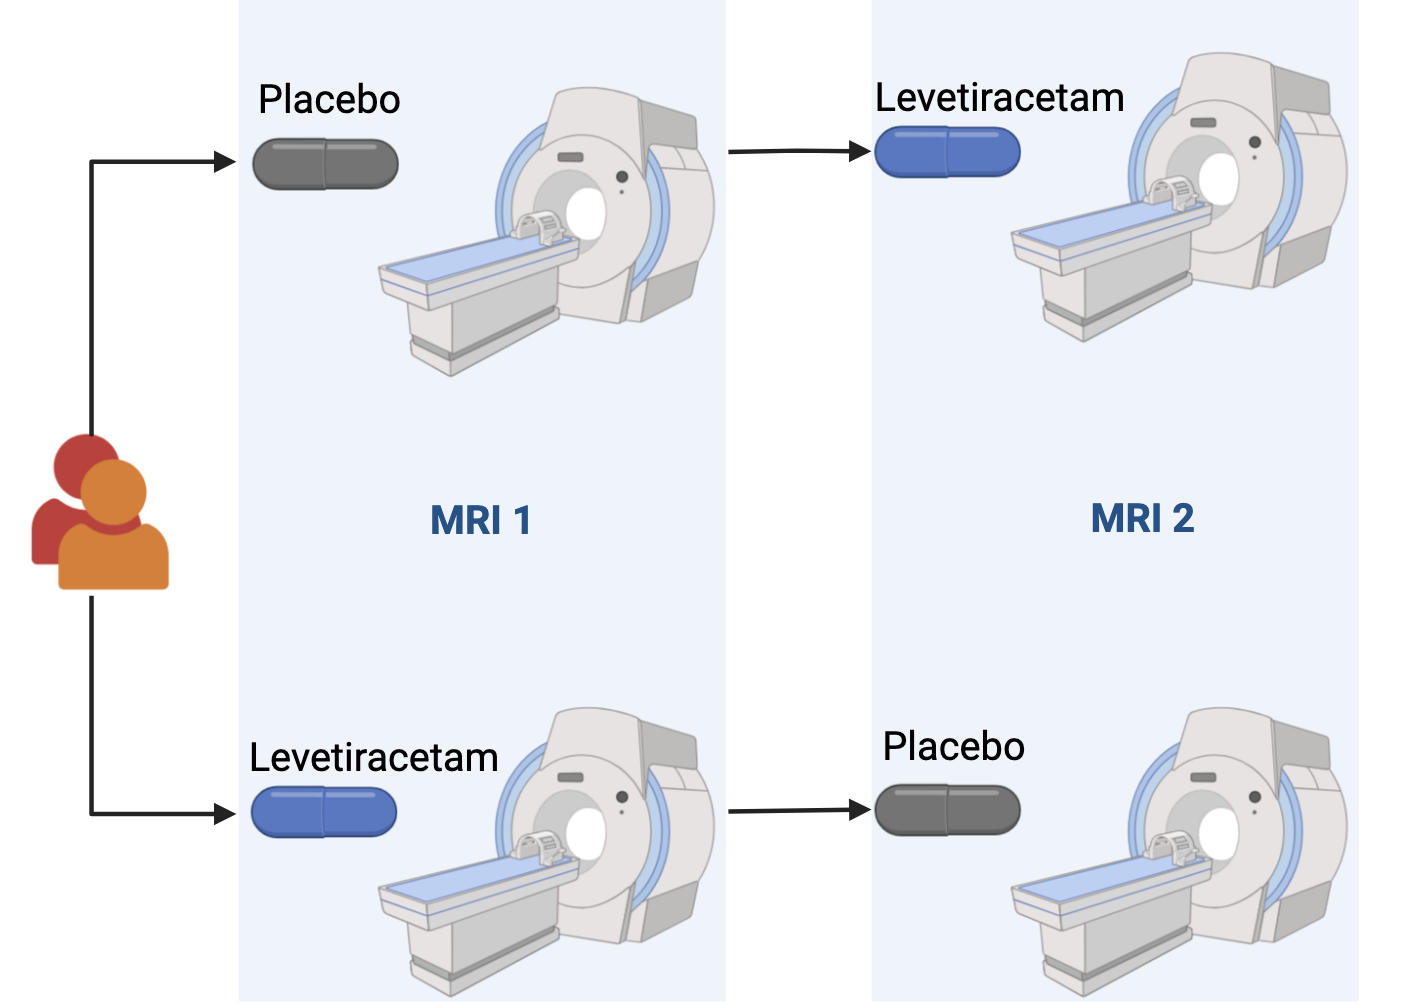
\includegraphics[width=0.75\textwidth,height=\textheight]{files/study_design.png}

}

\caption{\label{fig-study_design}Study design: participants are
randomised into the order in which they receive the placebo and
levetiracetam (HC= healthy controls, SZ=participatns with
schizophrenia)}

\end{figure}%

\subsubsection{Measuring glutamate}\label{measuring-glutamate}

\begin{itemize}
\tightlist
\item
  Glutamate levels in the ACC and the Hippocampus using single voxel
  spectroscopy (svs) PRESS sequence. The choice of those regions was
  based on previous findings of decreased SV2A density ({[}11C{]}UCB-J
  V\(_T\)) in the ACC in patients with schizophrenia
  \autocite{onwordi_synaptic_2020}, and altered relationship between
  glutamate and SV2A density in the hippocampus
  \autocite{onwordi_relationship_2021}.
\item
  I will also report Glx levels to verify if similar differences are
  observed compared to glutamate signal (This is due to limited ability
  to separate glutamine and glutamate using the PRESS sequence at 3T).
\end{itemize}

\subsubsection{Behavioural measures}\label{behavioural-measures}

\begin{itemize}
\tightlist
\item
  Change is symptoms is assessed using Positive and Negative Syndrome
  Scale (PANSS).
\item
  PANSS is administered at the screening appointment, and before and
  after every scan, to assess any change in symptoms related to
  levetiracetam.
\end{itemize}

\subsection{Analysis}\label{analysis}

\subsubsection{Change in glutamate}\label{change-in-glutamate}

\begin{itemize}
\tightlist
\item
  MRS data processing will be done in Osprey, and values corrected for
  partial volume efects for concentration of Glu (and Glx) will be
  extracted for each participant's scans.
\item
  To compare the changes in levels of glutamate between participants
  with schizophrenia and healthy controls I will do a 2x2 ANOVA.
\item
  I will also compare the concentration of glutamate at baseline between
  healthy controls and particiapnts with schizophrenia.
\item
  I will compare the effect of levetiracetam on Glx levels in healthy
  controls (HC) and patients with schizophrenia (SZ). This will be
  visualised on a raincloud plot such as the one below.
\item
  Below is example of data visualisation using a raincloud plot. The
  data used in this graph is made up. (I will add a plot with our data
  in the final version of the proposal)
\end{itemize}

\begin{figure}

\centering{

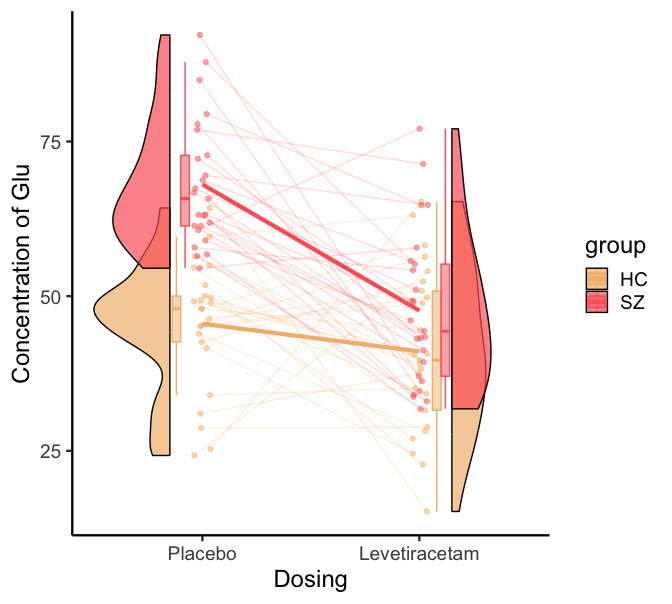
\includegraphics{index_files/figure-latex/notebooks-plots-fig-lev_hc_vs_sz-output-2.png}

}

\caption{\label{fig-lev_hc_vs_sz}Comparison of Glu levels change between
placebo and levetiracetam in HC and SZ}

\end{figure}%

\textsubscript{Source:
\href{https://juliam98.github.io/phd-upgrade-proposal/notebooks/plots-preview.html\#cell-fig-lev_hc_vs_sz}{Plots}}

\subsubsection{Change in symptoms}\label{change-in-symptoms}

\begin{itemize}
\tightlist
\item
  PANSS score for each symptom group and overall PANSS score will be
  calculated for all participants.
\end{itemize}

\section{Progress made to date, including pilot work, if
applicable}\label{progress-made-to-date-including-pilot-work-if-applicable}

\subsection{Progress with recruitment}\label{progress-with-recruitment}

So far the number of participants that completed the screening \&
baseline, and both MRI appointments in each group is:

\begin{itemize}
\tightlist
\item
  SZ: 11 (44\%)
\item
  HC: 5 (20\%)
\item
  \textbf{Total: 16 (32\%)}
\end{itemize}

I have been working on opening new research sites at 3 NHS trusts in
north London, where we will get support with recruitment from the local
research delivery teams. The first research site (CNWL) is expected to
open by the end of September 2024.

\subsection{Progress with analyses}\label{progress-with-analyses}

I am working on the setting up the data analysis pipeline for the MRS
data. I have been learning Osprey and wrote the code that I continue to
re-run once new data appears and troubleshoot any errors that come up.

\section{Planned future work}\label{planned-future-work}

\begin{itemize}
\tightlist
\item
  Continuing recruitment
\item
  Set up MRS preprocessing pipeline
\item
  ?
\end{itemize}

\section{Contribution to existing
knowledge.}\label{contribution-to-existing-knowledge.}

\textbf{How the research will form a distinct contribution to existing
knowledge on the subject and afford evidence of originality shown by
discovery of new facts or exercise of independent critical power}

This project will be the first one to examine the effects of modulating
SV2A with levetiracetam on glutamate levels in schizophrenia.It was
previously shown that SV2A density is decreased in schizophrenia
\autocite{radhakrishnan_vivo_2021,onwordi_synaptic_2020}, and that there
is an altered relationship between Glu and SV2A in schizophrenia. The
present study will provide more insight into the relationship between
glutamate levels and synaptic density in schizophrenia. Such findings
might have translational potential-

\section{Personal share in
investigations}\label{personal-share-in-investigations}

\textbf{Where work is done in conjunction with the supervisor and/or
with collaborators or other students, a statement of the candidate's own
personal share in the investigations}

I am jointly responsible for recruitment/data collection with other
student. I will do my analysis and write up independently.

\section{Timeline for the remainder of
studies.}\label{timeline-for-the-remainder-of-studies.}

\begin{itemize}
\tightlist
\item
  \textbf{Data collection}: October 2023 - Jan 2025
\item
  \textbf{Data analysis}: May 2024 - June 2026
\item
  \textbf{Write up}: November 2025 - January 2027
\item
  \textbf{Corrections to the manuscript}: January 2027 - April 2027
\item
  \textbf{Thesis submission}: May 2027
\item
  \textbf{Viva}: July 2027
\end{itemize}

\begin{figure}[H]

\centering{

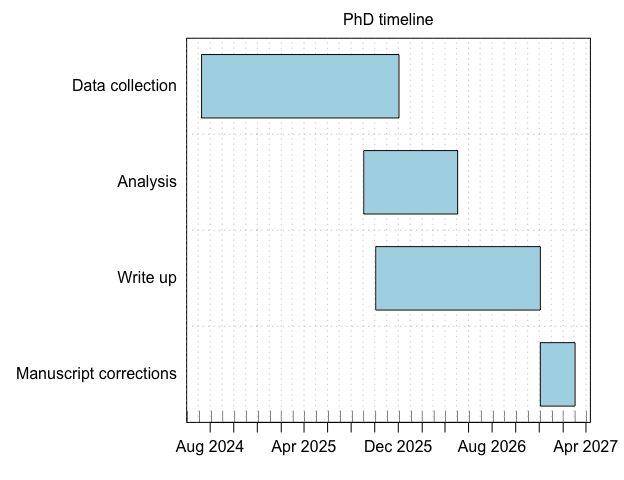
\includegraphics{index_files/figure-latex/notebooks-plots-fig-gantt-chart-output-1.png}

}

\caption{\label{fig-gantt-chart}Gantt chart of planned work during my
PhD}

\end{figure}%

\textsubscript{Source:
\href{https://juliam98.github.io/phd-upgrade-proposal/notebooks/plots-preview.html\#cell-fig-gantt-chart}{Plots}}

\newpage{}

\section{References}\label{references}

\printbibliography[heading=none]




\end{document}
